\chapter{Introduction}
\label{chap:introduction}

\section{About the project}

This thesis describes and documents the author's master's project, TTK4900, on underwater navigation. It was completed in partnership with Blueye Robotics AS. TTK4900 is worth 30 credits, with a project duration of 20 full-time weeks. The work presented in this thesis is an independent effort that is supervised by Professor Annette Stahl of NTNU and Johannes Schrimpf of Blueye via frequent status meetings.

\subsection{\acrshort{sonar} imaging}

\begin{figure}[H]
  \centering
  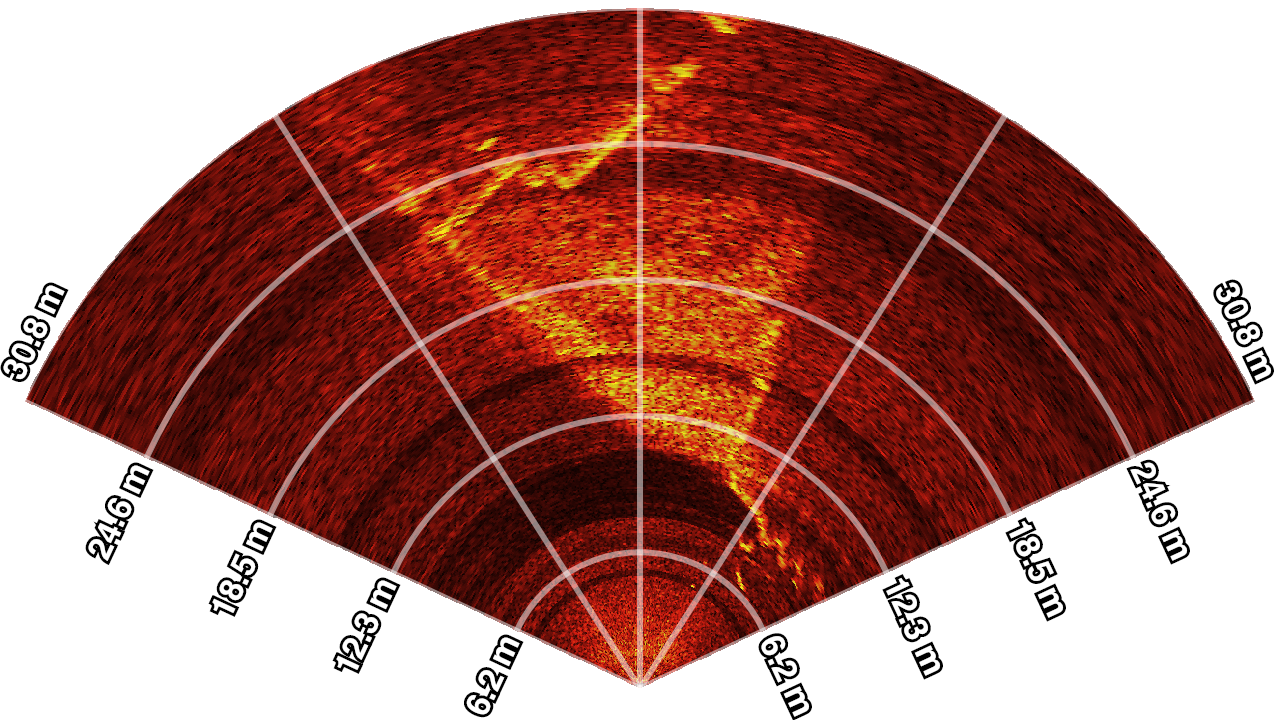
\includegraphics[width=.7\textwidth]{figures/sonar_processed.png}
  \caption[\acrshort{fls} image from \acrshort{bsosonar}]{Image obtained through a \acrfull{bsosonar} mounted on a Blueye Robotics X3 \acrshort{rov}}
  \label{fig:sonarapp}
\end{figure}

Underwater drones have revolutionized the way we explore underwater environments, providing unparalleled ease in accessing areas previously difficult to reach. However, visibility underwater is often severely limited, with cameras typically capturing images only within a few meters. To overcome this challenge, tools like \acrfull{fls}  are employed, allowing us to explore greater distances with relative ease. Despite its advantages, \acrshort{fls} is constrained by physical factors that result in noisy, inaccurate, and incomplete images, making the data difficult to interpret. From a single frame it may be very difficult to pick out useful information but given more information from a sequence of frames we can understand better what we see.

To address these challenges, image processing techniques can be applied to the frames recovered from \acrshort{fls}. Much research has gone into better visualization techniques of the covered area through mosaicing and noise reduction. And very interestingly image registration techniques may also allow for the estimation of the drone’s movement. In this thesis, I will implement an image processing pipeline that creates a mosaic of all the image frames and estimates odometry using data collected from a \acrfull{rov} equipped with \acrshort{fls}. This approach aims to enhance the clarity and usability of the \acrshort{sonar} data, ultimately improving the ability to navigate and understand underwater environments. If successfully implemented in real-time, the benefits to navigation using an \acrfull{rov} would be great. 

\section{The Project Proposal - Mosaicing \acrshort{fls} frames to aid in \acrshort{rov} navigation}

\begin{figure}[H]
  \centering
  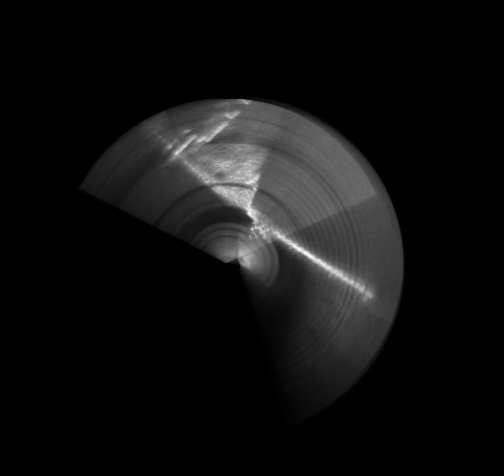
\includegraphics[width=.7\textwidth]{figures/example-output.png}
  \caption[Example mosaicing]{Mosaicing of \acrshort{bsosonar} frames captured on Blueye \acrshort{rov}}
  \label{fig:sonarapp}
\end{figure}

Being the product of collaboration with Blueye Robotics, the ultimate goal of the thesis is to make the \acrshort{sonar} data collected through the drone more useful. Together with Johanness Schrimpf and Jonas Follesoe from Blueye, we've identified registration and mosaicing of \acrshort{sonar} frames as a useful feature as in the future it might unlock some other applications:

\begin{itemize}
    \item Having a map of the areas covered with the drone to refer to might aid in navigation, exploration, and reporting.
    \item Being able to visualize things beyond the range of the \acrshort{sonar} all together in one image might make inspections easier.
    \item Could turn the \acrshort{fls} into a tool for bathymetry surveys, adding more functionality to existing tools on the drone.
    \item The transformations that describe the movement between one frame and the next one are also an indication of real movement of the drone. This odometry estimation might be useful for navigation and station keeping.
\end{itemize}

\subsection{Identified Tasks}
To meet the base goal of registering image pairs and generating \acrshort{sonar} mosaics certain tasks and goals must be met:

\begin{enumerate}
    \item Gather data for testing
        \begin{itemize}
            \item Generate fake data in a similar format to the \acrshort{sonar}
            \item Capture real data using an \acrshort{fls} mounted on a Blueye \acrshort{rov}
        \end{itemize}
    \item Process raw sensor data into \acrshort{sonar} images
    \item Implement a pipeline for image registration
        \begin{itemize}
            \item Compare different approaches to image registration
        \end{itemize}
    \item Implement an image stitching step that combines the images into a \acrshort{sonar} map
    \item Compare performance of different pipelines experimentally
\end{enumerate}

\section{Contributions}

After working on this thesis these are some of my contributions to the field:
\begin{itemize}
    \item Developing a flexible image registration pipeline framework.
    \item Developing a \acrshort{cli} application to generate seabed mosaics.
    \item Proposing improvements for a combined pipeline that might take advantage of the strengths of each of the pipelines proposed in the document. 
\end{itemize}


\section{Sustainability}

Some sustainability aspects that this thesis might have an impact on:

\begin{itemize}
    \item Reduce danger for divers: by being able to map the seabed, if there is a need to send down divers, they will have more data available to make more informed decisions about their dive beforehand.
    \item Reduce the need for additional positioning equipment on the drone: this work lays the bases for future development on the drone to be able to use the sonar as a positioning system. In lieu of a \acrshort{dvl}, the sonar could be used for station keeping or dead-reckoning. Additional work is required to get this operational, assuming fast enough computing on the drone to do this in real time. 
\end{itemize}


\section{Thesis Structure}

The following chapters of the thesis will be organized as follows:

\begin{itemize}
    \item \textbf{Chapter \ref{chap:background}}: introduces background theory necessary to understand \acrshort{fls}, it's image formation process, and theory behind registration pipelines.
    \item \textbf{Chapter \ref{chap:implementation}}: delves into the actual implementation of the pipeline and its sub-modules.
    \item \textbf{Chapter \ref{chap:setup}}: explains the experimental setup and preparation of the experiments for performance comparison.
    \item \textbf{Chapter \ref{chap:results}}: presents the results of the experiments to make it easier to compare the different pipelines.
    \item \textbf{Chapter \ref{chap:discussion}}: the discussion chapter contains an assessment of the results and implementations
    \item \textbf{Chapter \ref{chap:conclusion}}: the last chapter will demonstrate how successfully the objectives of the thesis are met. It concludes with a summary of the final results and recommendations for further work.
\end{itemize}

\section{Implementation overview}

\subsection{Tools and equipment}

A Blueye Robotics X3 \acrshort{rov} was provided by the company for the project's experiments. It comes equipped with a \acrfull{bsosonar} and a \acrfull{wldvl}. The \acrshort{bsosonar} is mounted on a skid that allows for tilt through a servo. The \acrshort{wldvl} allows the drone to maintain it's position in the water using the station-keeping mode while simultaneously providing dead-reckoning based positioning of the drone.

\begin{figure}[H]
  \centering
  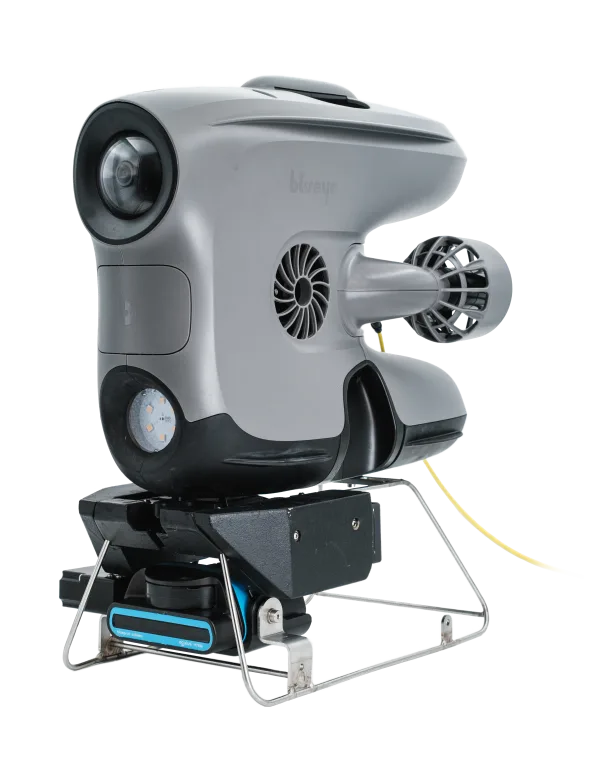
\includegraphics[width=.5\textwidth]{figures/blueye_x3.png}
  \caption[Blueye Robotics X3 \acrshort{rov} equipped with \acrshort{bsosonar}]{Equipment for experimentation provided by Blueye Robotics. Standard Blueye X3 drone equipped with a \acrshort{fls} and a \acrshort{dvl}. Image provided by Blueye \cite{Blueye:X3}.}
  \label{fig:sonarapp}
\end{figure}

On the software side, for ease of development the project uses Python as the main programming language, with extensive use of \href{https://numpy.org}{NumPy}, \href{https://scikit-image.org}{scikit-image} and \href{https://scipy.org}{scipy} for image processing and the implementation of the pipelines. In addition \href{https://www.ray.io}{Ray} is used for basic CPU parallelization. 

